\subsection{Blur Gaussiano}

\subsubsection{Descripción del filtro}

El filtro \textit{Blur Gaussiano}, produce un desenfoque en la imagen original
en base a un coeficiente $\sigma$ y \textit{r} entero. Estas variables son
parámetros que afectan por un lado, la dispersión o varianza de la distribución
normal de Gauss, y por el otro, la discretización de la misma. El uso de la
función de densidad de la distribución normal es clave para el resultado del
efecto ya que el mismo es el resultado de realizar un promedio ponderado de
los vecinos de cada pixel, tomando como pesos los valores discretizados de la
función.

Esto tiene una consecuencia directa sobre el resultado del filtro, y es que si
tomamos un $\sigma$ grande, implicando mayor dispersión, y utilizamos un
\textit{r} pequeño, veremos que la imagen producida se verá oscurecida (Figura \ref{fig:blur_s1_r1}), esto
se debe a que nuestra función de densidad integra a 1 cuando se recorren todos
sus valores, pero al discretizar, la suma no llega a 1, se está recortando gran
parte de la imagen de la función. Una posible solución es aumentar el radio,
obteniendo así más valores de la función y permitiendo que la suma vaya
aproximándose a 1 (Figura \ref{fig:blur_s1_r5}).

% TODO: generar las imágenes posta, esto es fruta

\begin{figure}[H]
	\centering
	\begin{minipage}{.3\textwidth}
		\centering
		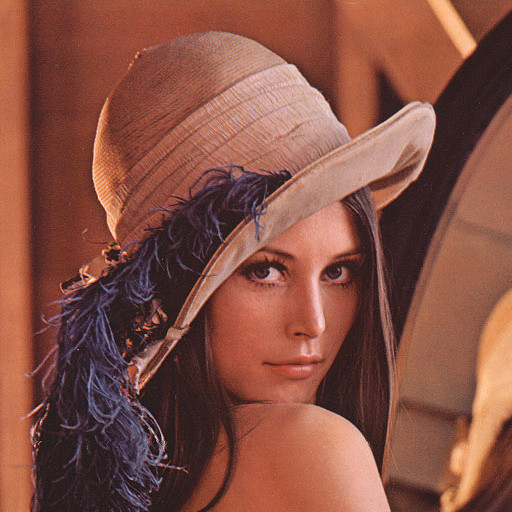
\includegraphics[width=\linewidth]{blur_original.jpg}
		\caption{Imagen original}
		\label{fig:blur_original}
	\end{minipage}\hfill
	\begin{minipage}{.3\textwidth}
		\centering
		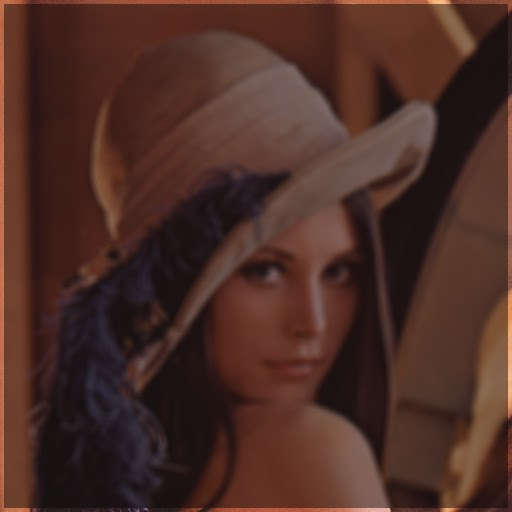
\includegraphics[width=\linewidth]{blur_s1_r1.jpg}
		\caption{Blur  $\sigma = 1, r = 1$}
		\label{fig:blur_s1_r1}
	\end{minipage}\hfill
	\begin{minipage}{.3\textwidth}
		\centering
		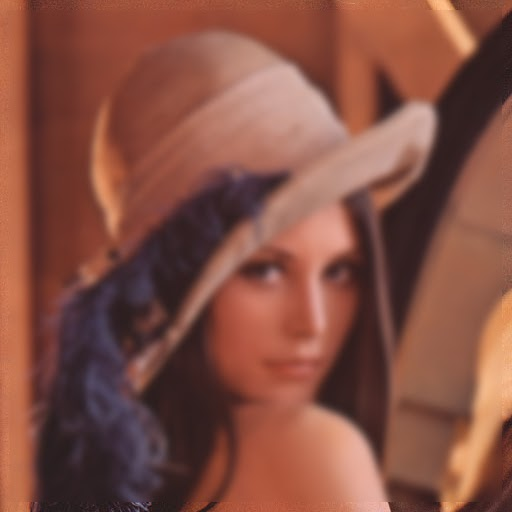
\includegraphics[width=\linewidth]{blur_s1_r5.jpg}
		\caption{Blur $\sigma = 1, r = 5$}
		\label{fig:blur_s1_r5}
	\end{minipage}
\end{figure}


A continuación se describirán las dos implementaciones que se realizaron en ASM
para lo cual antes comentaremos los principales componentes que aparecen
en las mismas. Por un lado tenemos las imágenes de entrada y la de salida, donde
comienzan siendo idénticas, y a medida que avanza el algoritmo, la de destino va
modificándose hasta llegar al resultado final. Por otra parte está la matriz de
convolución. Esta es de gran importancia, ya que es la que contiene todos los
coeficientes discretizados de la función de Gauss, y será la que al aplicarse
sobre los vecinos del pixel a procesar nos generará el promedio ponderado.

\subsubsection{Implementación de control}

Aquí desarrollaremos en detalle sobre la primer implementación en ASM, la de
control, cuya característica principal es mediante SIMD procesar de a pixeles
enteros las operaciones necesarias.

\subsubsection{Implementación experimental}

